\section{Azioni globali}
Di seguito le azioni che possono essere effettuate in qualsiasi modalità di creazione di diagrammi.

\subsection{Esportare Java}
Per salvare il progetto in uso, dal menu superiore, all'interno della voce "File" selezionare "Esporta".
\begin{figure}[h!]
	\centering
		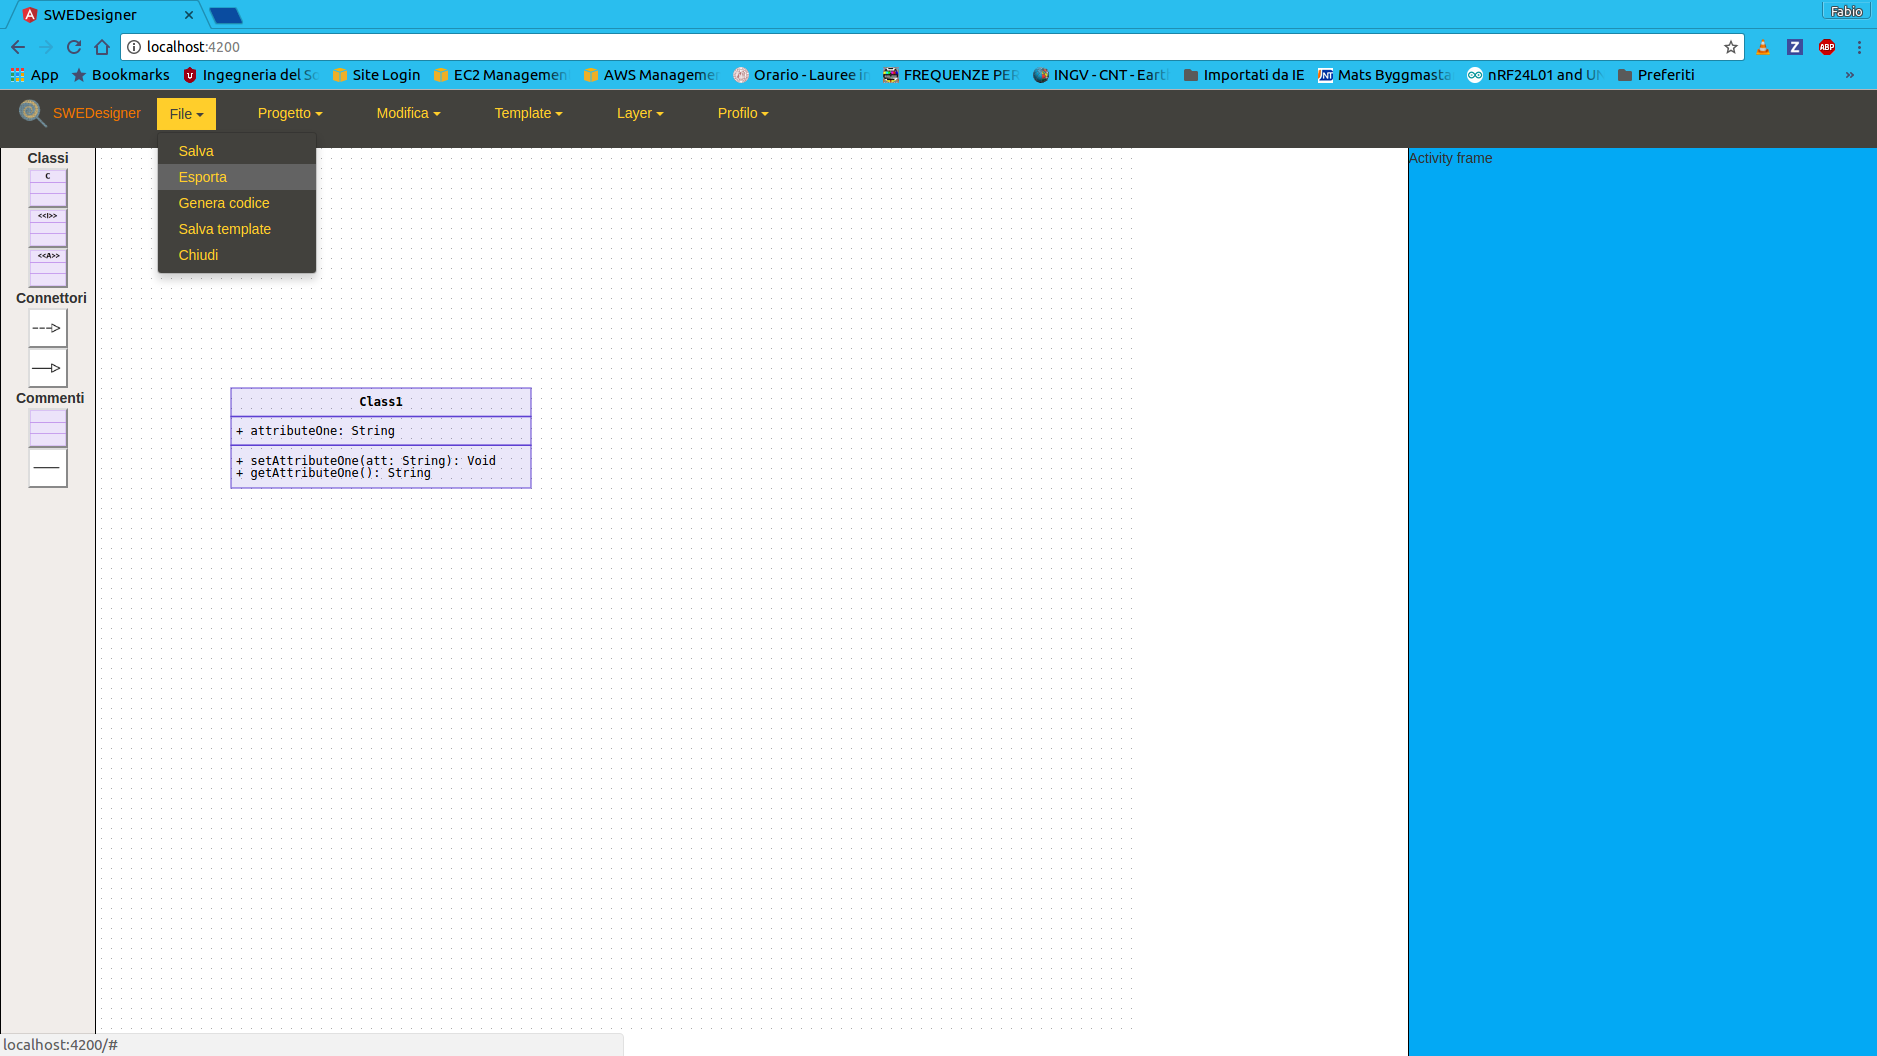
\includegraphics[scale=1]{../img/esporta.png}
	\caption{Esporta codice sorgente Java}
\end{figure}

\newpage

\subsection{Operazioni di Zoom}
Per effettuare le operazioni di zoom dei diagrammi selezionare dal menu superiore, all'interno della voce "Modifica" selezionare "Zoom In" oppure "Zoom Out".
\begin{figure}[h!]
	\centering
		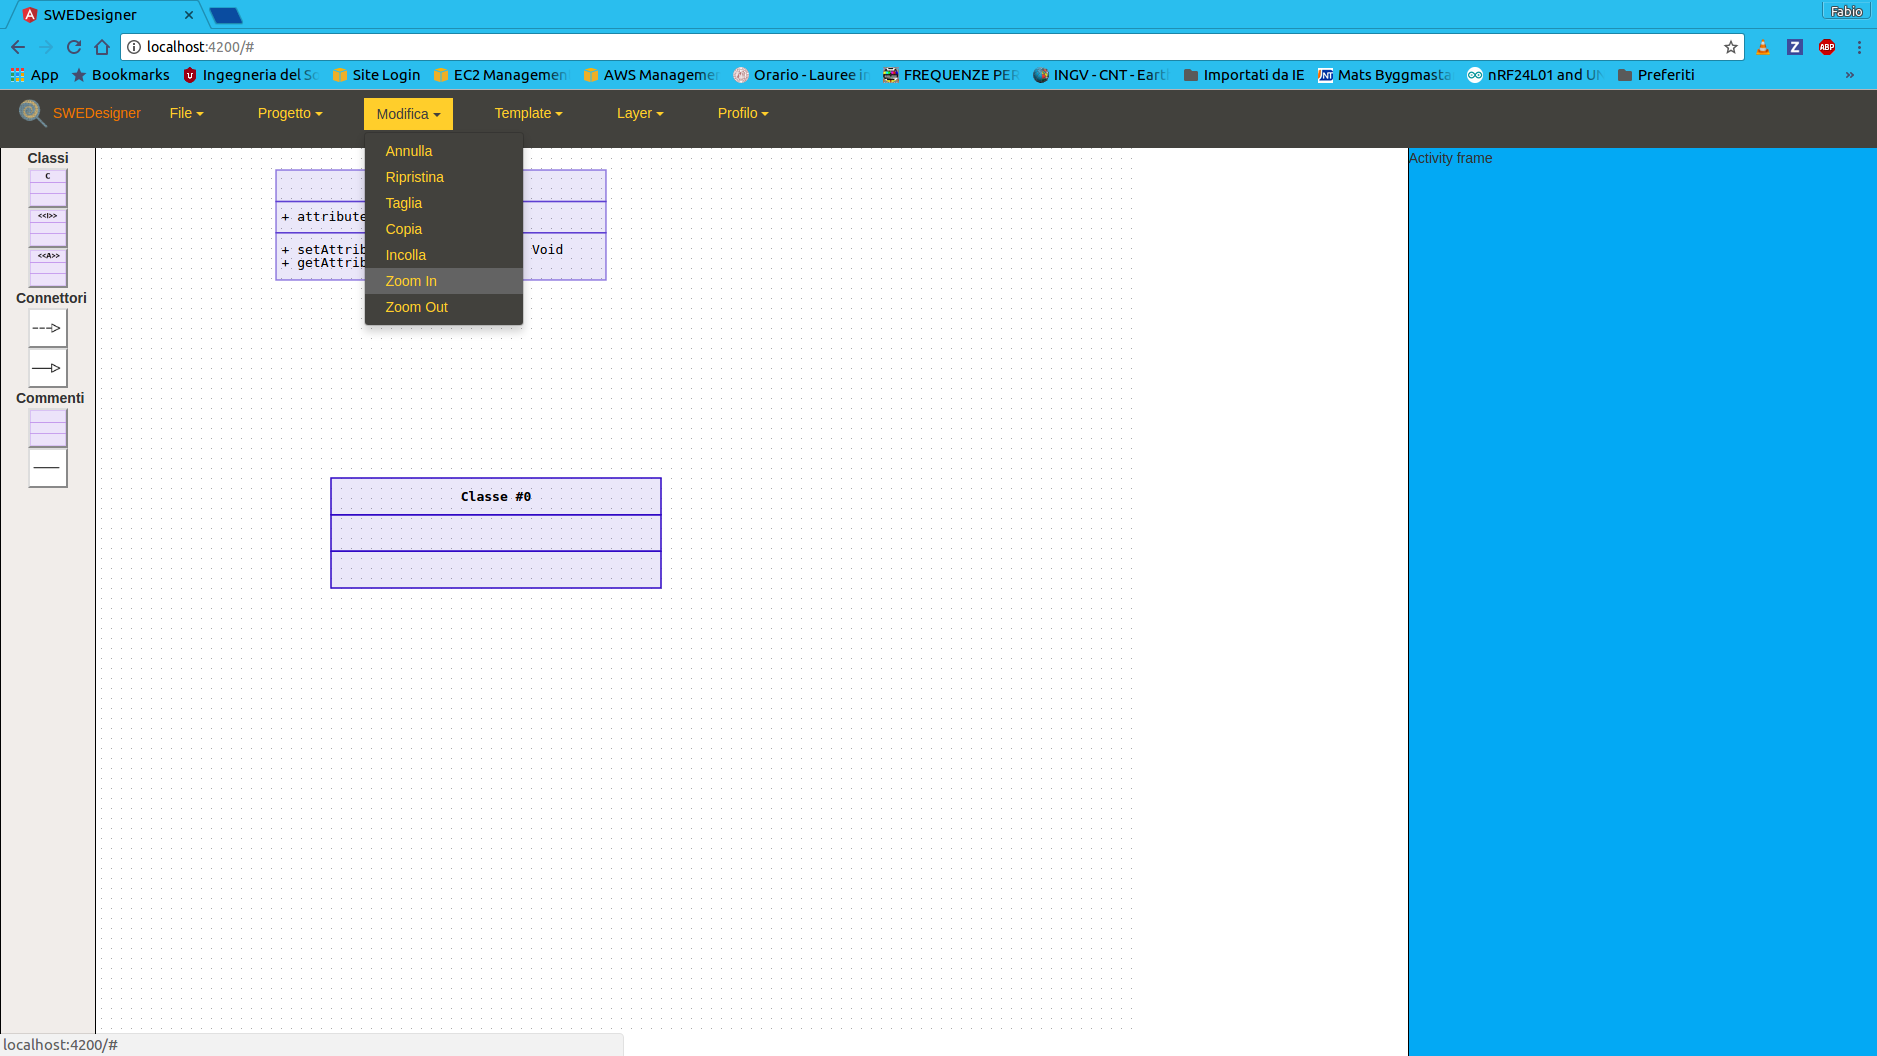
\includegraphics[scale=1]{../img/Zoom.png}
	\caption{Zoom}
\end{figure}
\newpage

\subsection{Eliminazione elemento}
Per eliminare un elemento disegnato, ma non desiderato, bisogna selezionare l'elemento, e dal menu superiore, all'interno della voce "Modifica" selezionare "Elimina".
\begin{figure}[h!]
	\centering
		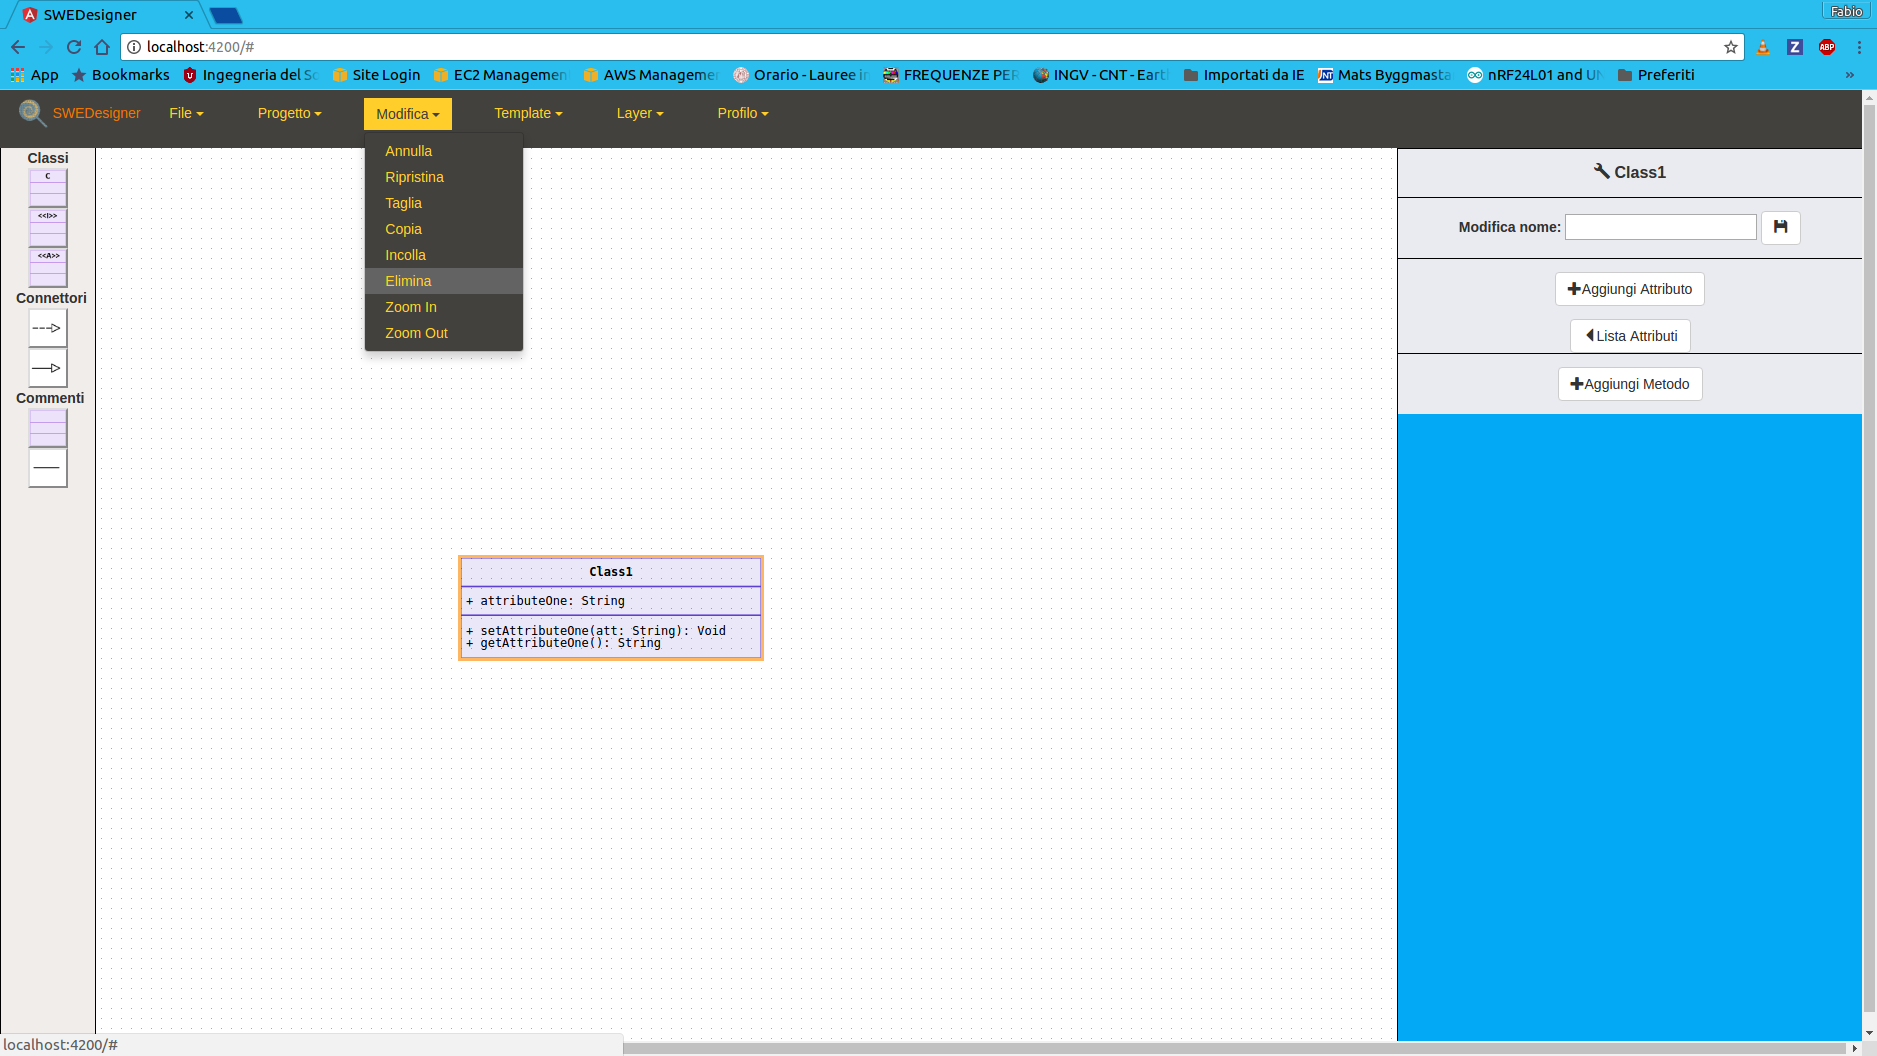
\includegraphics[scale=1]{../img/elimina.png}
	\caption{Elimina}
\end{figure}
\newpage

\subsection{Associazioni tra elementi}
Per realizzare una associazione tra due elementi, una volta selezionato il tipo di relazione dal menu laterale di sinistra, bisogna cliccare prima sul elemento di partenza e successivamente sul elemento di destinazione. In seguito verrà visualizzata la freccia rappresentante l'associazione tra gli elementi.
\begin{figure}[h!]
	\centering
		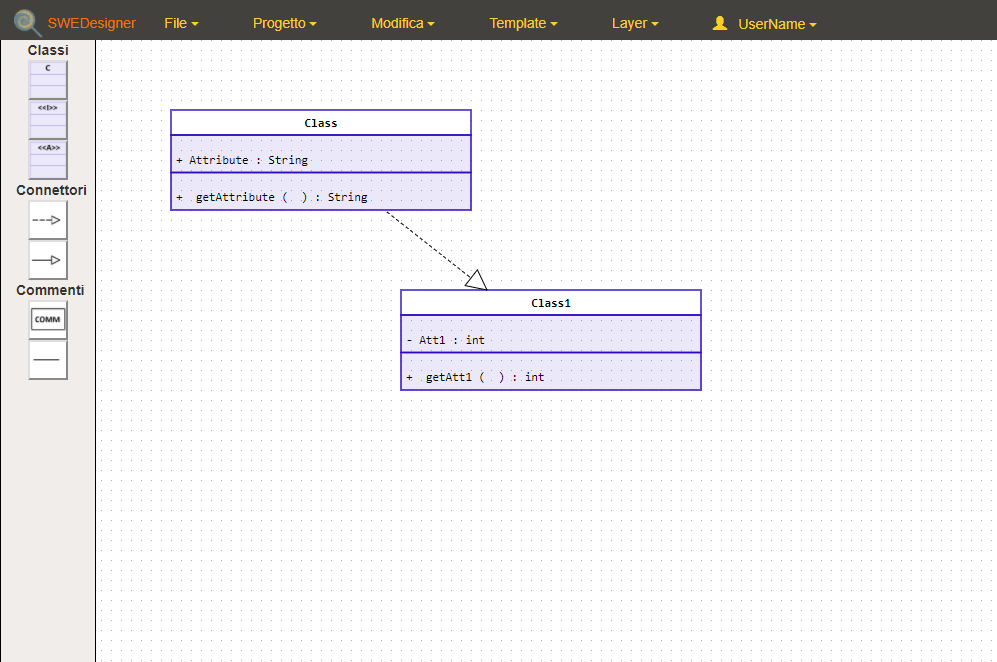
\includegraphics[scale=1]{../img/associazioneElementi.png}
	\caption{Associazione Elementi}
\end{figure}